\section{Gr\"obner Bases}

The contents here contained are a summary of the information provided in class with Chapter 2, sections 1-8 of \textit{Ideals, Varieties, and Algorithms} by Cox \textit{et. al}.

\subsection{Introduction}

\begin{definition}[Polynomial]
    A \textit{polynomial} $f$ in $x_1, \dots, x_n$ with coefficients in a field $k$ is a finite linear combination (with coefficients in $k$) of monomials.
    The set of all polynomials in $x_1, \dots, x_n$ with coefficients in $k$ is denoted $k[x_1, \dots, x_n]$.
\end{definition}

\begin{definition}[Affine Space]
    Given a field $k$ and a positive integer $n$, we define the $n$-dimensional \textit{affine space} over $k$ to be the set
    $$k^n = \{ (a_1, \dots, a_n) | a_1, \dots, a_n \in k \}$$
\end{definition}

\begin{definition}[Affine Variety]
    Let $k$ be a field and let $f_1, \dots, f_s$ be polynomials in $k[x_1, \dots, x_n]$.
    Then the affine variety defined by $f_1, \dots, f_s$ is,
    $$\pmb{V}(f_1, \dots, f_s) = \{ (a_1, \dots, a_n) \in k^n | f_i(a_1, \dots, a_n) = 0 \quad \forall 1 \leq i \leq s \}$$
\end{definition}

\begin{definition}[Ideals]
    A subset $I \subseteq k[x_1, \dots, x_n]$ is an \textit{ideal} if it satisfies:
    \begin{enumerate}
        \item[(i)] $0 \in I$
        \item[(ii)] If $f, g \in I$, then $f + g \in I$
        \item[(iii)] If $f \in I$ and $h \in k[x_1, \dots, x_n]$ then $hf \in I$.
    \end{enumerate}
    Additionally, let $f_1, \dots, f_s$ be polynomials in $k[x_1, \dots, x_n]$.
    Then,
    $$<f_1, \dots, f_s> = \left\{ \sum_{i=1}^s h_i f_i | h_1, \dots, h_s \in k[x_1, \dots, x_n] \right\}$$
    is the \textit{ideal generated} by $f_1, \dots, f_s$.

    Lastly, if $V \subseteq k^n$ is an affine variety, the set
    $$\pmb{I}(V) = \{f \in k[x_1, \dots, x_n] | f(a_1, \dots, a_n) = 0 \quad \forall (a_1, \dots, a_n) \in V\}$$
    is \textit{the ideal of V}.
\end{definition}

\subsection{Orderings on the Monomials}

\begin{definition}[Monomial Ordering]
    A \textit{monomial ordering} > on $k[x_1, \dots, x_n]$ is a relation $>$ on $\Z^n_{\geq 0}$, or equivalently, a relation on the set if monomials $x^{\alpha}$, $\alpha \in \Z^n_{\geq 0}$, satisfying:
    \begin{enumerate}
        \item[(i)] $>$ is a total (or linear) ordering on $\Z^n_{\geq 0}$
        \item[(ii)] If $\alpha > \beta$ and $\gamma \in \Z^n_{\geq 0}$, then $\alpha + \gamma > \beta + \gamma$.
        \item[(iii)] $>$ is a well-ordering on $\Z^n_{\geq 0}$.
            This means that every nonempty subset of $\Z^n_{\geq 0}$ has a smallest element under $>$.
    \end{enumerate}
\end{definition}

\begin{definition}[Lexicographical Order]
    Let $\alpha = (\alpha_1, \dots, \alpha_n)$ and $\beta = (\beta_1, \dots, \beta_n)$ be in $\Z^n_{\geq 0}$.
    We say $\alpha >_{lex} \beta$ if the leftmost nonzero entry of the vector difference $\alpha - \beta \in \Z^n$ is positive.
    We will write $x^{\alpha} >_{lex} x^{\beta}$ if $\alpha >_{lex} \beta$.
\end{definition}

\begin{definition}[Graded Lex Order]
    Let $\alpha, \beta \in \Z^n_{\geq 0}$.
    We say $\alpha >_{grlex} \beta$ if
    $$|\alpha| = \sum_{i=1}^n \alpha_i > |\beta| = \sum_{i=1}^n \beta_i, \quad or \quad |\alpha | = | \beta | \text{ and } \alpha >_{lex} \beta$$
\end{definition}

\begin{definition}[Graded Reverse Lex Order]
    Let $\alpha, \beta \in \Z^n_{\geq 0}$.
    We say $\alpha >_{grlex} \beta$ if
    $$|\alpha| = \sum_{i=1}^n \alpha_i > |\beta| = \sum_{i=1}^n \beta_i, \quad or \quad |\alpha | = | \beta | \text{ and the rightmost nonzero entry of } \alpha - \beta \text{ is negative }$$
\end{definition}

\begin{theorem}[Division Algorithm]
    Let $>$ be a monomial order on $\Z^n_{\geq 0}$ and let $F = (f_1, \dots, f_s)$ be an ordered $s$-tuple of polynomials in $k[x_1, \dots, x_n]$.
    Then, every $f \in k[x_1, \dots, x_n]$ can be written as:
    $$f = q_1f_1 + \dots + q_sf_s + r$$
    where $q_i, r \in k[x_1, \dots, x_n]$, and either $r = 0$ or it is a linear combination, with coefficients in $k$, of monomials none of which is divisible by any of $LT(f_1), \dots, LT(f_s)$.
    The algorithm is depicted in Figure~\ref{fig:division-algorithm}.
\end{theorem}
\begin{figure}[h!]
    \centering
    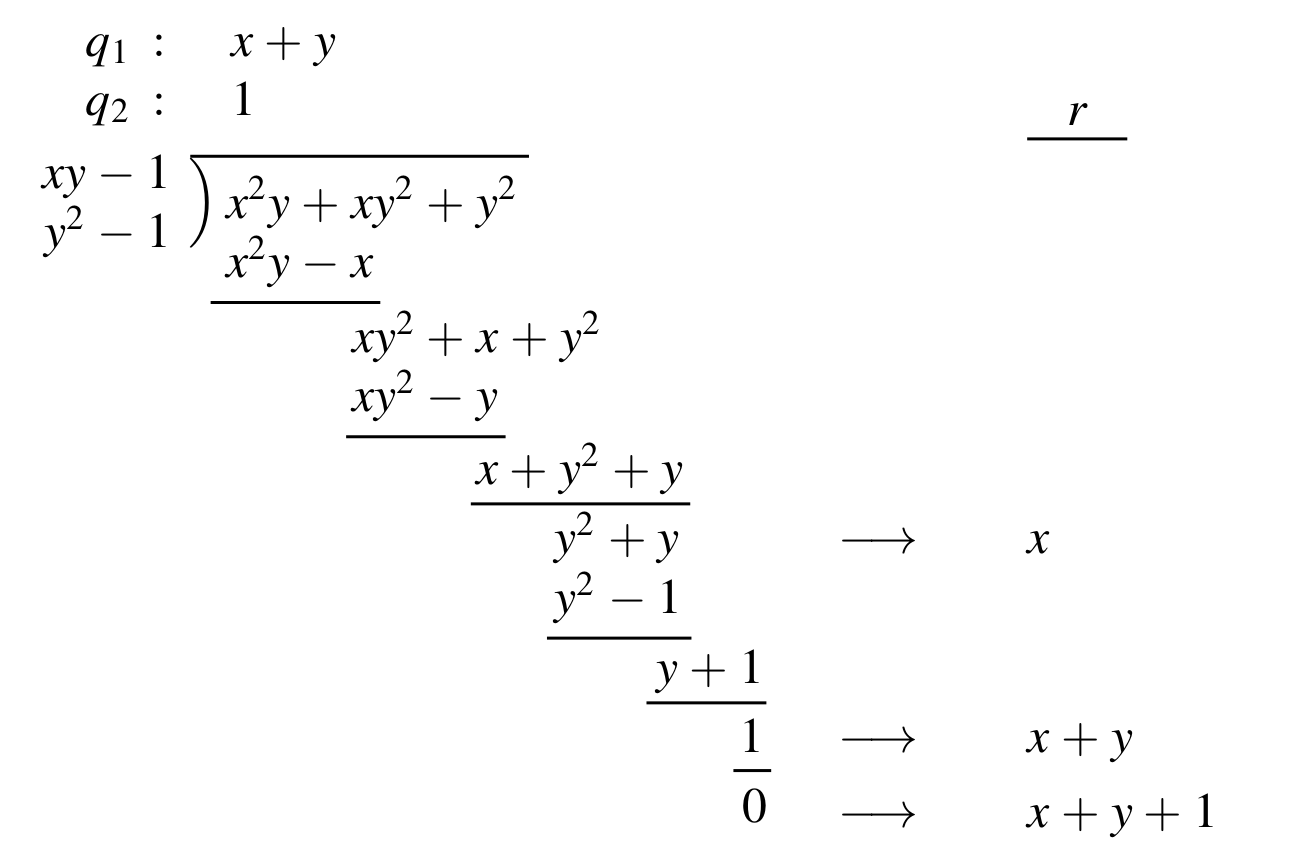
\includegraphics[width=.6\textwidth]{img/division.png}
    \caption{Division algorithm for polynomials.\label{fig:division-algorithm}}
\end{figure}

Note that, with the defined division algorithm, we can check for ideal membership by dividing by all the ideal generators and checking the remainder (sufficient, but not necessary). I.e. depending on the order we give to $(f_1, \dots, f_s)$ the remainder may vary.
Gr\"obner bases will solve this problems.
